%----------------------------------------------------------------------%
% Trajectory analysis code "Tacode" version 2: Theory, Verification and Validation
% Yusuke Takahashi, Hokkaido University
% English version (authoritative)
%----------------------------------------------------------------------%
\documentclass[11pt,a4paper]{article}

\usepackage{graphicx}
\usepackage{amsmath, amsfonts, amssymb}
\usepackage{array}
\usepackage{url}
\usepackage{fancyhdr}
\usepackage{listings}
\usepackage[margin=25mm]{geometry}
\usepackage[hidelinks]{hyperref}

\graphicspath{ {./figure/} }

\pagestyle{fancy}
\fancyhf{}
\rhead{\thepage}
\lhead{Tacode version 2: Theory, Verification and Validation}

\lstset{%
  basicstyle={\small\ttfamily},
  backgroundcolor={\color[gray]{.95}},
  frame=single,
  breaklines=true,
  columns=fullflexible,
  xleftmargin=2em,
  xrightmargin=0em,
  lineskip=-0.3ex
}
\usepackage{color}

\newcommand{\bx}{{\boldsymbol x}}
\newcommand{\bv}{{\boldsymbol v}}
\newcommand{\bF}{{\boldsymbol F}}
\newcommand{\bM}{{\boldsymbol M}}
\newcommand{\bI}{{\boldsymbol I}}
\newcommand{\bq}{{\boldsymbol q}}
\newcommand{\bOm}{{\boldsymbol \Omega}}
\newcommand{\bom}{{\boldsymbol \omega}}
\newcommand{\bC}{{\boldsymbol C}}
\newcommand{\bR}{{\boldsymbol R}}

%----------------------------------------------------------------------%
\begin{document}

\begin{center}
{\Large \bf Trajectory Analysis Code ``Tacode'' Version 2 \\[2mm]
Theory, Verification and Validation}
\end{center}

\begin{center}
{\normalsize
  Yusuke Takahashi\footnote{E-mail: ytakahashi@eng.hokudai.ac.jp} \\
  {\itshape Hokkaido University, Kita 13 Nishi 8, Kita-ku, Sapporo, Hokkaido 060-8628, Japan}
}
\end{center}

\begin{abstract}
\noindent
Tacode is a trajectory analysis code that integrates the equations of motion of a point
mass, and since version 2.3 of a rigid body, in the Earth-Centered Earth-Fixed rotating
frame. Version 1 of this manuscript described the three-degree-of-freedom formulation and
the operation of the code. This report describes version 2: the six-degree-of-freedom
extension, the lift force and the bank angle, the wind field, the absolute time, and the
numerical safeguards that were added with them. It then reports what has been done to
establish that the code is correct. Verification is by a suite of 488 automated tests
built on closed-form solutions, physical identities and mutation testing; the observed
order of convergence of the time integration is measured. Validation is against three
flights: Apollo 4 (1967), Apollo 10 (1969) and Project Fire flight II (1965). The last of
these is treated at length, because it is the only flight found that can exercise the
attitude solver against measured data, and because the reasoning that went into deciding
what it can and cannot establish is itself part of the result.
\end{abstract}

%----------------------------------------------------------------------
\section*{Nomenclature}
\begin{tabbing}
\hspace{4.0em}\= \hspace{1.5em} \= \hspace{11cm} \kill
	$a_e$      \> = \> semi-major axis (equatorial radius), m \\
	$C_D, C_L$ \> = \> drag and lift coefficients \\
	$C_{F}, C_{M}$ \> = \> force and moment coefficients in body axes \\
	$C_{lp}, C_{mq}, C_{nr}$ \> = \> dynamic damping derivatives, 1/rad \\
	$\bC_{b/e}$ \> = \> transformation matrix from ECEF to body axes \\
	$d$        \> = \> reference diameter, m \\
	$e$        \> = \> first eccentricity \\
	$f$        \> = \> ellipticity \\
	$\bF$      \> = \> force vector, N \\
	$G$        \> = \> gravitational constant, m$^3$/kg$\cdot$s$^2$ \\
	$H$        \> = \> altitude in the geodetic system, m \\
	$\bI$      \> = \> inertia tensor about the centre of gravity, kg m$^2$ \\
	$J$        \> = \> dynamic form factor \\
	$Kn$       \> = \> Knudsen number \\
	$L$        \> = \> characteristic length, m \\
	$m$        \> = \> mass of the vehicle, kg \\
	$M$        \> = \> mass of the planet, kg \\
	$\bM$      \> = \> moment vector, N m \\
	$p, q, r$  \> = \> body-axis components of the angular velocity relative to ECEF, rad/s \\
	$q_{\infty}$ \> = \> dynamic pressure, N/m$^2$ \\
	$\bq$      \> = \> attitude quaternion, scalar first \\
	$r$        \> = \> radial distance in the polar system, m \\
	$\bR_x$    \> = \> rotation matrix about the body $x$ axis \\
	$S$        \> = \> characteristic area, m$^2$ \\
	$t$        \> = \> time, s \\
	$U$        \> = \> gravitational potential, m$^2$/s$^2$ \\
	$\bv$      \> = \> velocity vector in the ECEF frame, m/s \\
	$\bx$      \> = \> position vector in the ECEF frame, m \\
	$\alpha$   \> = \> longitude in the polar system, rad; also angle of attack, rad \\
	$\alpha_t$ \> = \> total angle of attack, rad \\
	$\beta$    \> = \> latitude in the polar system, rad; also sideslip angle, rad \\
	$\eta$     \> = \> total angle of attack, deg (the notation of the Fire reports) \\
	$\lambda$  \> = \> longitude in the geodetic system, rad \\
	$\rho$     \> = \> atmospheric density, kg/m$^3$ \\
	$\sigma$   \> = \> bank angle, rad \\
	$\phi$     \> = \> latitude in the geodetic system, rad \\
	$\varphi_a$ \> = \> aerodynamic roll angle, rad \\
	$\bom$     \> = \> angular velocity vector of the planet, rad/s \\
	$\bOm$     \> = \> angular velocity of the body relative to the inertial frame, rad/s \\
	$\bOm_{\rm rel}$ \> = \> angular velocity of the body relative to the ECEF frame, rad/s \\
\end{tabbing}

%----------------------------------------------------------------------
\section{Introduction}

The trajectory of a spacecraft sets the environment every other discipline has to design
for: the dynamic pressure, the heat flux, the time spent in orbit and the dispersion of
the landing point. A trajectory tool is therefore needed early and used often, and it is
worth more if it is simple to drive, easy to couple to other tools, and honest about what
it does and does not model.

Version 1 of Tacode, described in the preceding manuscript, integrated the three
translational degrees of freedom of a point mass in the rotating frame of a planet, with
gravity expanded in spherical harmonics, the Coriolis and centrifugal terms of the
rotating frame, and a drag force read from a tabulated atmosphere. That is enough for a
ballistic entry or a launch, and it is what the code was used for.

It is not enough for three things that came up afterwards. A blunt entry capsule flies
with lift, and the direction of that lift --- the bank angle --- is what a guidance system
commands; without it the computed trajectory of a lifting entry is not wrong by a few per
cent but by tens of kilometres. The attitude of an uncontrolled body oscillates, and the
period and amplitude of that oscillation are the design quantities for a spin-stabilised
probe; a point mass has nothing to say about them. And a re-entry that ends in the
troposphere drifts downwind, which a co-rotating atmosphere cannot represent.

Version 2 adds all three, together with an absolute time so that date-dependent models can
be driven, and a set of numerical safeguards. Table \ref{version_history} lists what
arrived when.

\begin{table}[h]
\caption{What each version of Tacode 2 added. Every new model is off by default, and with
it off the output is unchanged byte for byte, which the regression tests enforce.}
\label{version_history}
\begin{center}
\begin{tabular}{l|l}
\hline \hline
Version & Added \\
\hline
2.0 -- 2.2 & Python implementation of the version 1 formulation \\
2.3.0 & Six degrees of freedom: attitude quaternion, Euler equations, aerodynamic table in $\alpha_t$ \\
2.3.1 & Warning when a tabulated aerodynamic database is not axisymmetric \\
2.4.0 & Wind field, and an absolute epoch \\
2.5.0 & Lift and bank angle in three degrees of freedom; divergence detection; \\
      & Monte-Carlo failure detection and random seed; validation against flight data \\
\hline \hline
\end{tabular}
\end{center}
\end{table}

The second half of this report is about correctness rather than capability. A trajectory
code is easy to write and hard to trust: its output is plausible over a wide range of
wrong coefficients, and a sign error in a term that is normally small is invisible until
the case that makes it large. Section \ref{verification} describes the verification
strategy --- comparison with closed-form solutions, physical identities, mutation testing,
and byte-for-byte regression --- and Section \ref{validation} the comparison with three
actual flights.

%----------------------------------------------------------------------
\section{Mathematical Model}

\subsection{State vector and degrees of freedom}

Tacode advances a state vector in the Earth-Centered Earth-Fixed (ECEF) rotating frame of
Figure \ref{cartesian_coordinate}. In three degrees of freedom the state is the position
and the velocity of a point mass. Setting \texttt{attitude.flag\_attitude: True} adds the
attitude quaternion and the angular velocity of a rigid body:
%
\begin{align}
	{\boldsymbol y} = \left[ \bx, \; \dot{\bx} \right] \quad \textrm{(3-DOF)} ,
	\qquad
	{\boldsymbol y} = \left[ \bx, \; \dot{\bx}, \; \bq, \; \bOm \right] \quad \textrm{(6-DOF)} .
\end{align}
%
Both sets are advanced by the same integrator with the same time step. The translational
and rotational equations are coupled in both directions: the moments turn the body, and
the aerodynamic force follows the attitude. Of the forces below only the aerodynamic one
depends on the attitude, so with the attitude switched off the translational set reduces
\emph{exactly} to the three-degree-of-freedom equations of version 1.

\begin{figure}[h]
\begin{center}
	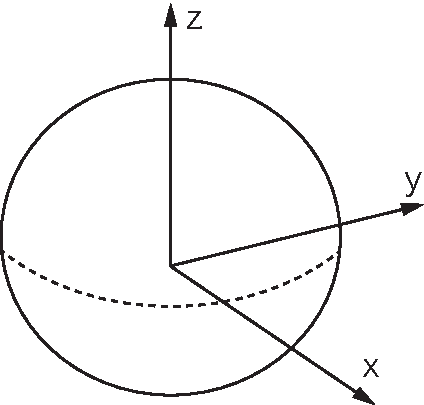
\includegraphics[width=0.30\linewidth]{cartesian_coordinate}
\end{center}
\caption{The Cartesian (ECEF) coordinate system.}
\label{cartesian_coordinate}
\end{figure}

\subsection{Translational motion}

The equation of motion of a mass point in the non-inertial ECEF frame is
%
\begin{align}
	m \frac { \partial^{2} \bx }{ \partial t^{2} } =
	\bF_{\rm grav}
	- 2 m \bom \times \frac { \partial \bx }{ \partial t }
	- m \bom \times \left( \bom \times \bx \right)
	+ \bF_{\rm aero} ,
	\label{law_momentum}
\end{align}
%
where $t$ is time, $\bx$ and $m$ are the position vector and the mass, and $\bom$ is the
angular velocity of the frame. For the Earth,
$\bom = (0, 0, 7.292115\times10^{-5})$ rad/s. The second and third terms on the right are
the Coriolis and centrifugal forces that appear because the frame rotates; at the equator
the centrifugal term is about 1\,\% of gravity.

\subsection{Rotational motion}

The rotation of the rigid body about its centre of gravity is governed by Euler's
equation, written in body axes where the inertia tensor is constant:
%
\begin{align}
	\bI \frac{ \partial \bOm }{ \partial t }
	+ \bOm \times \left( \bI \bOm \right)
	= \bM_{\rm aero} + \bM_{\rm damp} + \bM_{\rm grav} .
	\label{law_euler}
\end{align}
%
Here $\bOm$ is the angular velocity \emph{with respect to the inertial frame}, expressed
in body components, and the three moments on the right are the aerodynamic, the dynamic
damping and the gravity-gradient moments, each of which can be switched off individually.

\subsection{Coordinate systems}

Four frames are used, and the conventions matter enough to state them together.

\begin{itemize}
\item The \textbf{ECEF Cartesian frame} (Figure \ref{cartesian_coordinate}) is where the
equations are integrated. The $x$ axis passes through longitude $0$, the $y$ axis through
longitude $90^\circ$ and the $z$ axis through the poles.
\item The \textbf{geodetic system} (Figure \ref{geodetic_coordinate}) gives latitude
$\phi$, longitude $\lambda$ and altitude $H$ on the WGS84 spheroid; it is how the initial
position is given and how the result is written out. With
$N = a_e / \sqrt{1 - e^2 \sin^2\phi}$ and $e^2 = f(2-f)$,
\begin{align}
	X = (N+H) \cos\phi \cos\lambda , \quad
	Y = (N+H) \cos\phi \sin\lambda , \quad
	Z = \left[ N(1-e^2) + H \right] \sin\phi ,
\end{align}
with $a_e = 6.3781370 \times 10^6$ m and $f = 1/298.257223563$ for the Earth. The inverse
is solved by the closed-form Bowring-type iteration.
\item The \textbf{geocentric polar system} (Figure \ref{geodetic_coordinate}, right),
with radius $r$, longitude $\alpha$ and latitude $\beta$, is where the gravity is
evaluated.
\item The \textbf{local horizon} is a geocentric north-east-down frame, and the
\textbf{body frame} is [forward, right, down]. The Euler angles that Tacode reads and
writes are a 3-2-1 (yaw, pitch, roll) sequence from the local horizon to the body frame,
with yaw measured from north towards east.
\end{itemize}

\begin{figure}[h]
\begin{center}
	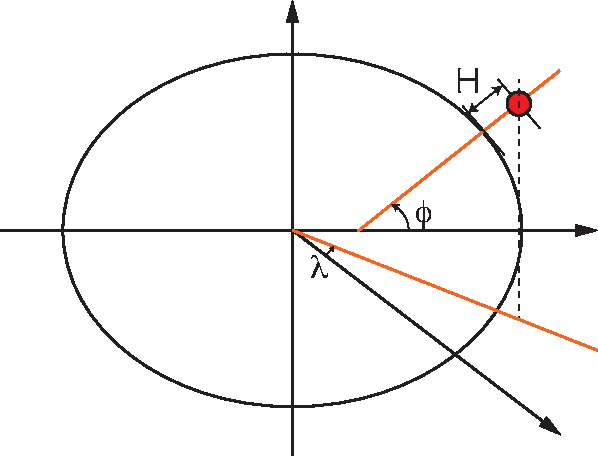
\includegraphics[width=0.28\linewidth]{geodetic_coordinate}
	\hspace{12mm}
	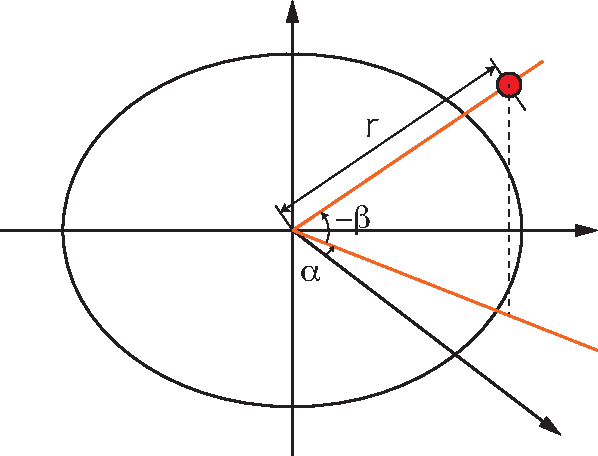
\includegraphics[width=0.28\linewidth]{polar_coordinate}
\end{center}
\caption{The geodetic system (left) and the geocentric polar system (right).}
\label{geodetic_coordinate}
\end{figure}

\textbf{One convention is worth repeating because it catches people.} The initial position
is \emph{geodetic} while the initial velocity is given in the \emph{geocentric} local
horizon [east, north, up], and so is the wind. The two verticals differ by up to
$0.19^\circ$. The code is self-consistent --- the output is geocentric too --- but a state
vector taken from an external source has to be converted, and the validation cases in
Section \ref{validation} each carry a script that does exactly that.

\subsection{Gravity}

Because the planet is a spheroid, the potential is expanded in spherical harmonics in the
polar frame \cite{Wagner1966,Liu2019}:
%
\begin{align}
	U = - \frac{G M}{r}
	\left[ 1
	- \left( \frac{a_{e}}{r} \right)^2 J_{20} \frac{ 3 \sin^2 \beta - 1}{2}
	- \left( \frac{a_{e}}{r} \right)^2 J_{22} \, 3 \cos^2 \beta \cos 2 \left( \alpha + \alpha_{22} \right) \right.
	\nonumber \\
	\left.
	- \left( \frac{a_{e}}{r} \right)^3 J_{30} \frac{ 5 \sin^3 \beta - 3 \sin \beta}{2}
	- \left( \frac{a_{e}}{r} \right)^4 J_{40} \frac{1}{8} \left( 35 \sin^4 \beta - 30 \sin^2 \beta + 3 \right) \right] ,
\end{align}
%
whose gradient in polar components gives $\bF_{\rm grav}$, which is then rotated into the
Cartesian frame. Figure \ref{potential_schematic} shows what the terms represent: the
equipotential surface departs from a sphere, and each $J$ term is one mode of that
departure. The parameters used for the Earth are in Table \ref{J_parameters}; they are
configuration entries, so another planet is a matter of changing them and supplying an
atmosphere table.

\begin{figure}[h]
\begin{center}
	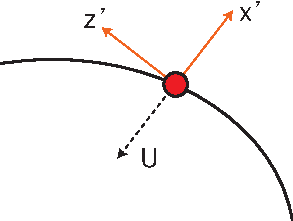
\includegraphics[width=0.30\linewidth]{potential_schematic}
\end{center}
\caption{The equipotential surface of a rotating spheroid, which the expansion in $J$
terms describes.}
\label{potential_schematic}
\end{figure}

\begin{table}[h]
\caption{Dynamic form factors used for the Earth (\texttt{planet.potential\_factor}).}
\label{J_parameters}
\begin{center}
\begin{tabular}{l|r|l|r}
\hline \hline
Parameter & Value & Parameter & Value \\
\hline
$J_{20}$ & $1.082629 \times 10^{-3}$   & $J_{40}$ & $-1.62336 \times 10^{-6}$ \\
$J_{22}$ & $-1.81222 \times 10^{-6}$   & $\alpha_{22}$ & $-14.545$ deg \\
$J_{30}$ & $-2.5356 \times 10^{-6}$    & $GM$ & $3.98600 \times 10^{14}$ m$^3$/s$^2$ \\
\hline \hline
\end{tabular}
\end{center}
\end{table}

\subsection{Aerodynamic force}

The dynamic pressure is $q_{\infty} = \frac{1}{2} \rho \left| \bv_{\rm air} \right|^2$,
where $\bv_{\rm air}$ is the velocity relative to the air. With the wind off, the
atmosphere co-rotates with the planet and $\bv_{\rm air} = \bv$.

\paragraph{Three degrees of freedom.}
The attitude is unknown, so the force is a drag along the direction of motion,
%
\begin{align}
	\bF_{\rm drag} = - q_{\infty} C_D S \frac{ \bv_{\rm air} }{\left| \bv_{\rm air} \right|} ,
\end{align}
%
optionally with a lift perpendicular to it, whose direction in that plane is set by the
bank angle $\sigma$ (Figure \ref{body_axes}, right):
%
\begin{align}
	\bF_{\rm lift} = q_{\infty} C_L S \left( \cos\sigma \, \hat{\boldsymbol n}_u + \sin\sigma \, \hat{\boldsymbol n}_r \right) ,
	\quad
	\hat{\boldsymbol n}_u = \frac{ \hat{\boldsymbol u} - ( \hat{\boldsymbol u} \cdot \hat{\bv} ) \hat{\bv} }{ \left| \cdot \right| } ,
	\quad
	\hat{\boldsymbol n}_r = \hat{\bv} \times \hat{\boldsymbol n}_u ,
	\label{lift}
\end{align}
%
with $\hat{\boldsymbol u} = \bx / |\bx|$ the local (geocentric) vertical. So $\sigma = 0$
is lift up and $\sigma = 180^\circ$ lift down. Tacode carries no guidance law: the bank
angle is either a constant or a table against time, which is how a \emph{measured} roll
history is flown. Each Runge-Kutta stage reads the table at its own time. With
$C_L = 0$ the lift is not evaluated at all, so a configuration without it reproduces the
version-1 result bit for bit.

\paragraph{Six degrees of freedom.}
The force is read from a table in body axes as a function of the total angle of attack and
the Knudsen number. Writing $[u, v, w] = \bC_{b/e} \bv_{\rm air}$ for the air-relative
velocity in body components (Figure \ref{body_axes}, left),
%
\begin{align}
	\alpha_t = \arccos \frac{u}{\left| \bv_{\rm air} \right|} , \qquad
	\varphi_a = \arctan \frac{v}{w} ,
\end{align}
%
where $\alpha_t$ is the angle between the body $x$ axis and the velocity and $\varphi_a$
is the angle between the plane the coefficients were tabulated in and the plane the
crossflow actually lies in. The table is entered at $\alpha_t$ and rotated about the body
$x$ axis onto that plane,
%
\begin{align}
	\bF_{\rm aero} = - q_{\infty} S \, \bC_{F} ,
	\qquad
	\bC_{F} = \bR_{x} \left( \varphi_a \right)
	\begin{bmatrix} C_{Fx} \\ C_{Fy} \\ C_{Fz} \end{bmatrix} \left( \alpha_t, Kn \right) ,
	\label{force_6dof}
\end{align}
%
which is \emph{exact} for a body of revolution --- which is what a table indexed by
$\alpha_t$ alone describes. A table that is not axisymmetric is reported at load time
rather than used silently. The sign is chosen so that at zero incidence
$\bC_F = [C_D, 0, 0]$ and Eq. (\ref{force_6dof}) reduces to the three-degree-of-freedom
drag; the two formulations therefore agree to the last bit at $\alpha_t = 0$, and the test
suite checks that they do.

\begin{figure}[h]
\begin{center}
	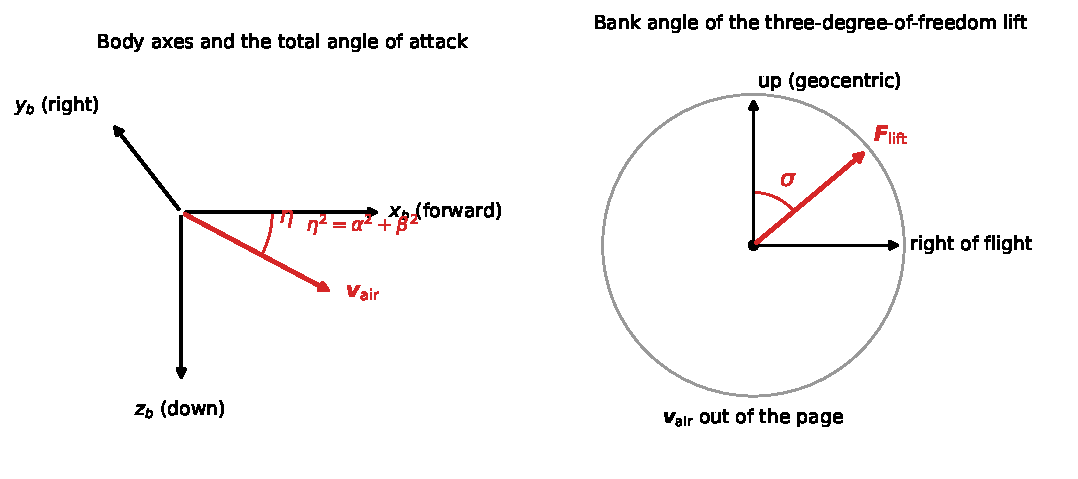
\includegraphics[width=0.92\linewidth]{body_axes}
\end{center}
\caption{Left: the body axes and the total angle of attack $\eta = \alpha_t$. Right: the
bank angle $\sigma$ of the three-degree-of-freedom lift, in the plane perpendicular to the
air-relative velocity.}
\label{body_axes}
\end{figure}

\subsection{Aerodynamic, damping and gravity-gradient moments}

The moment coefficients are read from the same table at the same $\alpha_t$ and rotated by
the same $\bR_x(\varphi_a)$ --- a proper rotation, so the pseudo-vector of the moment
transforms exactly as the force does --- and are then transferred from the reference point
of the table to the centre of gravity:
%
\begin{align}
	\bM_{\rm aero} = q_{\infty} S L \, \bC_{M}
	+ \left( {\boldsymbol r}_{\rm ref} - {\boldsymbol r}_{\rm cg} \right) \times \bF_{\rm aero} ,
	\qquad
	\bC_{M} = \bR_{x} \left( \varphi_a \right)
	\begin{bmatrix} C_{Mx} \\ C_{My} \\ C_{Mz} \end{bmatrix} \left( \alpha_t, Kn \right) .
	\label{moment_aero}
\end{align}
%
With the body axes [forward, right, down] a positive $C_{My}$ pitches the nose up, so a
statically stable body has $C_{My} < 0$ at a positive angle of attack.

The table gives static coefficients, that is, the moment on a body held at a fixed
attitude. A rotating body also feels a moment opposing its rotation:
%
\begin{align}
	\bM_{\rm damp} = q_{\infty} S L \frac{L}{2 \left| \bv_{\rm air} \right|}
	\begin{bmatrix} C_{lp} \, p \\ C_{mq} \, q \\ C_{nr} \, r \end{bmatrix} .
	\label{moment_damp}
\end{align}
%
Without it the oscillation of a statically stable body never decays, because the static
coefficients alone are conservative. Finally, the first-order effect of the gradient of
gravity across the body is
%
\begin{align}
	\bM_{\rm grav} = \frac{3 G M}{r^3} \, \hat{\boldsymbol u} \times \left( \bI \hat{\boldsymbol u} \right) ,
	\qquad
	\hat{\boldsymbol u} = \bC_{b/e} \frac{ \bx }{ \left| \bx \right| } ,
\end{align}
%
which vanishes for an isotropic inertia tensor and whenever a principal axis is aligned
with $\hat{\boldsymbol u}$. For a small vehicle in low Earth orbit it is of order
$10^{-6}$ N m --- negligible against the aerodynamic moment during an entry, but the only
moment left in vacuum.

\subsection{Attitude kinematics, and the two angular velocities}

The attitude is carried by a quaternion $\bq = [q_0, q_1, q_2, q_3]$ (scalar first)
representing the transformation from ECEF to body axes,
${\boldsymbol z}_b = \bC_{b/e} {\boldsymbol z}_e$. A quaternion is used rather than the
Euler angles themselves because it has no singularity: an entry body passing through a
pitch of $90^\circ$ would hit the gimbal lock of a 3-2-1 sequence. Its evolution is
%
\begin{align}
	\frac{ \partial \bq }{ \partial t } = \frac{1}{2} {\boldsymbol Q} \left( \bOm_{\rm rel} \right) \bq ,
	\qquad
	{\boldsymbol Q} = \begin{bmatrix}
	0 & -p & -q & -r \\
	p & 0 & r & -q \\
	q & -r & 0 & p \\
	r & q & -p & 0 \end{bmatrix} .
\end{align}
%
\textbf{Two angular velocities appear and they must not be confused.} Euler's equation
(\ref{law_euler}) is written for the rate with respect to the \emph{inertial} frame,
$\bOm$, whereas the quaternion is referred to the rotating ECEF frame and evolves with
%
\begin{align}
	\bOm_{\rm rel} = \left[ p, q, r \right] = \bOm - \bC_{b/e} \bom .
\end{align}
%
Leaving the planetary rate in would drift the attitude by $0.0042$ deg/s. The same
relative rate is the one the aerodynamic damping (\ref{moment_damp}) sees, because the
atmosphere co-rotates. The quantity integrated is $\bOm$; the input in the configuration
file and the output in the result file are both $\bOm_{\rm rel}$, which is the more
intuitive of the two, so the code converts at the boundaries. The quaternion is
renormalised at every stage of the integration.

\subsection{Wind}

The wind relaxes the assumption that the atmosphere co-rotates rigidly with the planet:
%
\begin{align}
	\bv_{\rm air} = \bv - \bv_{\rm wind} ({\rm ECEF}) .
\end{align}
%
\textbf{Only the aerodynamics see it} --- the drag, the six-degree-of-freedom force and
moment, the dynamic pressure, the aerodynamic angles. Gravity, the Coriolis and
centrifugal terms and the angular velocity are untouched, because the wind is a
translational quantity and not a rotation of the frame. The wind is given in the
geocentric local horizon [east, north, up], the same frame as the initial velocity; that
differs from the geodetic frame of meteorological $u$/$v$ data by up to $0.19^\circ$, and
the choice was made so that the code carries one convention rather than two. When the
wind is off, the subtraction is not performed at all and the result is bit-for-bit that of
the earlier formulation.

\subsection{Absolute time}

An epoch may be attached to the initial condition. Nothing in the point-mass formulation
needs it, but a wind table with a time axis does, and it is the foundation for any
date-dependent model. The epoch is written into the header of the result file rather than
as a column, because the output format cannot carry a string in a data row. Leap seconds
are not considered, and there is at present no ECEF-to-ECI transformation.

%----------------------------------------------------------------------
\section{Discretised Model}

\subsection{Time integration}

Writing the right-hand side of Eq. (\ref{law_momentum}) as $\bF$ and of
Eq. (\ref{law_euler}) as the corresponding angular accelerations, the system is a set of
first-order equations advanced either by the explicit Euler method,
%
\begin{align}
	\bx^{n+1} = \bx^{n} + \bv^{n} \Delta t , \qquad
	\bv^{n+1} = \bv^{n} + \bF^{n} \Delta t ,
	\label{euler}
\end{align}
%
which is first-order accurate, or by the four-stage fourth-order Runge-Kutta method,
%
\begin{align}
&	{\boldsymbol k}_1 = {\boldsymbol f} \left( t^n, {\boldsymbol y}^n \right) \Delta t , \qquad
	{\boldsymbol k}_2 = {\boldsymbol f} \left( t^n + \tfrac{1}{2}\Delta t, {\boldsymbol y}^n + \tfrac{1}{2}{\boldsymbol k}_1 \right) \Delta t , \nonumber \\
&	{\boldsymbol k}_3 = {\boldsymbol f} \left( t^n + \tfrac{1}{2}\Delta t, {\boldsymbol y}^n + \tfrac{1}{2}{\boldsymbol k}_2 \right) \Delta t , \qquad
	{\boldsymbol k}_4 = {\boldsymbol f} \left( t^n + \Delta t, {\boldsymbol y}^n + {\boldsymbol k}_3 \right) \Delta t , \\
&	{\boldsymbol y}^{n+1} = {\boldsymbol y}^{n} + \tfrac{1}{6} \left( {\boldsymbol k}_1 + 2 {\boldsymbol k}_2 + 2 {\boldsymbol k}_3 + {\boldsymbol k}_4 \right) . \nonumber
\end{align}
%
The same stages advance the attitude, with the quaternion renormalised after each. The
time step is constant.

Two details are worth recording because they are easy to get wrong. First, the
\textbf{wind and the bank-angle table are read at the time of each stage}, with the stage
factors $[0, \frac{1}{2}, \frac{1}{2}, 1]$, not at the time of the step; anything else
silently reduces the order. Second, the atmospheric quantities that appear in the
\textbf{output} are those of the first stage, that is, evaluated at the reported position;
writing out the fourth-stage values would shift them by one step.

\subsection{Order of accuracy}

Figure \ref{order_of_accuracy} measures the observed order on the Project Fire II entry of
Section \ref{fire2}, a case that passes through a deceleration of 73 $g$. The state is
compared at a fixed time to a run at the finest step. The slope over the three finest
steps is $4.3$ for the position in three degrees of freedom and $3.9$ for the attitude
quaternion in six --- the fourth order of the scheme in both cases.

Two things about that figure are worth saying out loud. The coarse end of each curve
\emph{leaves} the fourth-order line, because the step there does not resolve the
deceleration peak or the attitude oscillation; the asymptotic range has to be found, not
assumed. And the interpolation of the tabulated data limits what can be reached: the
angle-of-attack table is only $C^0$, so a case whose incidence sweeps across table nodes
converges at an order between two and three rather than four, which the test suite
measures separately.

\begin{figure}[h]
\begin{center}
	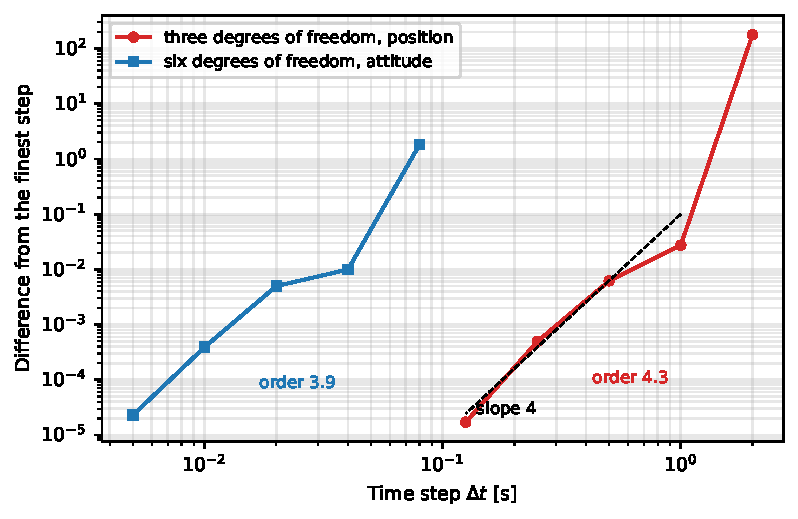
\includegraphics[width=0.62\linewidth]{order_of_accuracy}
\end{center}
\caption{Observed order of convergence on the Project Fire II entry. The difference from
the run at the finest step is plotted at a fixed time; the dashed line has slope 4. The
ordinate is a distance in metres for the three-degree-of-freedom series and the norm of
the quaternion difference for the six-degree-of-freedom one.}
\label{order_of_accuracy}
\end{figure}

\subsection{Time step for the attitude}

The period of the oscillation of a statically stable body,
%
\begin{align}
	T = 2 \pi \sqrt{ \frac{I_{yy}}{ q_{\infty} S L \left| C_{m\alpha} \right| } } ,
	\label{period}
\end{align}
%
shortens as the dynamic pressure rises, so a step that resolves the attitude at entry may
not resolve it at the peak. There is no sub-cycling; instead the solver checks
$\Delta t > T/20$ and warns once. The check is made once per second of simulated time
rather than every step: the dynamic pressure changes on a scale of seconds, and evaluating
it every step cost 9\,\% of a six-degree-of-freedom run.

\subsection{Divergence detection}

A trajectory integrated with too coarse a step does not stop --- it leaves the planet, and
the result file is written as though nothing were wrong. Version 2.5 builds limits from
the \emph{initial} state (ten times the geocentric distance, ten times the escape velocity
there) and checks the position, the velocity and, in six degrees of freedom, the
quaternion and the angular velocity once per step. A state that is not finite, or beyond a
limit, stops the run with an explicit message and a non-zero exit code. Limits relative to
the initial state rather than absolute ones are used because the meaning of ``too far''
depends on the orbit. A sound run never touches them.

%----------------------------------------------------------------------
\section{Models and Data}

\subsection{Atmosphere}

The atmosphere is a table of altitude against number densities, mass density and
temperature, read at run time; the models themselves live in generator scripts so that the
solver has no dependency on them. Two file formats are recognised and distinguished by
their content. The Knudsen number is formed from the number densities of N$_2$, O$_2$,
N and O and the characteristic length, and is what the aerodynamic table is indexed by.

Above the top of the table the density is extrapolated exponentially with a scale height
fitted to the measured profile over the top 50 km; the alternative is to clamp, which was
the version 2.1.1 behaviour. \textbf{The exponential is cut off at 100 scale heights}:
without a limit the exponential underflows and a density of exactly zero, with an infinite
Knudsen number, reaches the output. Below the bottom of the table the value is clamped.

Tables are generated with NRLMSISE-00 through \texttt{pymsis}, for a given date, position
and set of solar indices. The generator is the only thing that depends on \texttt{pymsis},
which is therefore not a requirement of the code.

\subsection{Aerodynamic coefficients}

Three levels are available. A \textbf{constant} drag coefficient needs no table at all. A
\textbf{table against the Knudsen number} gives $C_D(Kn)$ for three degrees of freedom. A
\textbf{table against the total angle of attack and the Knudsen number} gives the six
coefficients $C_{Fx}, C_{Fy}, C_{Fz}, C_{Mx}, C_{My}, C_{Mz}$ needed for six degrees of
freedom; it is organised in blocks introduced by a line \texttt{AOA <value>}, and a file
without such a line is read as a single block at zero incidence, which is why a version-1
table still reproduces a version-1 result exactly.

A generator builds such a table for a body of revolution by a panel method: modified
Newtonian theory on the continuum side, complete momentum exchange on the free-molecular
side, and a $\sin^2$ bridging function in the Knudsen number between $10^{-3}$ and $10$.
Two shapes are provided, a sphere-cone and an Apollo-type capsule; only the function that
draws the generatrix differs between them. A measured table can of course be supplied
instead, and in Section \ref{fire2} one is.

\subsection{Wind}

A wind table has up to four axes --- time, longitude, latitude, altitude --- and is read
in a single format. Longitudes are folded into $[-180, 180)$ and a global table is joined
across the seam by adding a wrapped node. The horizontal is always clamped; the vertical
follows a configurable rule whose default is zero, because the reanalysis data usually
available stop at about 31 km. A table with a time axis requires an epoch, and the run
stops if there is none rather than guessing. A scale factor multiplies the whole field,
which is how the Monte-Carlo driver disperses a tabulated wind.

%----------------------------------------------------------------------
\section{The Code}

Tacode 2 is written in Python 3 and depends on \texttt{numpy}, \texttt{scipy},
\texttt{PyYAML} and \texttt{simplekml}; \texttt{matplotlib} is optional and used only by
the post-processing tools. The solver is driven by a single YAML control file read from
the current directory, so a case is a directory:

\begin{lstlisting}
cd tutorial/work_reentry && ./run_tacode.sh
\end{lstlisting}

The state is passed between modules as dictionaries of history arrays --- Cartesian,
geodetic and polar positions; Cartesian and polar velocities; density, temperature and
Knudsen number; and, in six degrees of freedom, the quaternion and the angular velocity.
The attitude dictionary is updated in place inside the solver rather than returned, which
keeps the number of return values fixed between the two modes.

\textbf{The interpolators are built once.} The atmosphere, the aerodynamic table and the
wind each construct their interpolating object at initialisation and the accessors only
evaluate it. Rebuilding them per call, which an earlier version did, dominated the run
time.

Beyond the solver the distribution carries a Monte-Carlo driver, which copies a template
case, rewrites the requested entries of its control file as text so that comments survive,
runs the cases, detects those that fail, and gathers the results into one file with one
zone per case; and a set of post-processing tools for dispersion statistics and
animation, which read the solver's output but never run it.

%----------------------------------------------------------------------
\section{Verification} \label{verification}

\subsection{Strategy}

Verification here means establishing that the equations of Section 2 are solved correctly,
as distinct from establishing that they describe the flight. Four kinds of check are used,
and they were chosen because each has actually caught something.

\begin{enumerate}
\item \textbf{Closed-form solutions.} Conservation of energy and angular momentum in the
two-body limit; the Jacobi-elliptic solution of the torque-free asymmetric rigid body; the
precession rate of an axisymmetric body; the period of a linear pitch oscillation; the
logarithmic decrement of a damped one; the libration frequency of a gravity-gradient
stabilised body in a circular orbit. To guard against transcribing a reference solution
wrongly, the elliptic-function case is accompanied by a test that substitutes the claimed
solution back into Euler's equations and differentiates it numerically.
\item \textbf{Physical identities.} The aerodynamics under a wind $\boldsymbol{w}$ at
velocity $\bv$ must equal the aerodynamics in still air at $\bv - \boldsymbol{w}$. The
force and moment on an axisymmetric body must be unchanged, in ECEF components, when the
body is rolled about its own axis. The gravity vector must equal $-\nabla U$ for a
potential written independently of the solver. The six-degree-of-freedom force at zero
incidence must equal the three-degree-of-freedom drag.
\item \textbf{Mutation testing.} A coefficient or a sign is deliberately broken and the
suite must fail. This is applied to every new test, because it has repeatedly exposed
tests that passed for the wrong reason.
\item \textbf{Byte-for-byte regression.} A refactor that is not meant to change the answer
is accepted only if the output files are identical. Two regression cases, one with the
attitude off and one with it on, reproduce reference outputs committed with the code.
\end{enumerate}

\subsection{The test suite}

The suite comprises 488 tests in 20 modules and runs in about 55 seconds using only the
standard library's \texttt{unittest}. Table \ref{test_modules} groups them. A separate
smoke test runs a tutorial case end to end in a temporary directory and inspects the
output files. Continuous integration runs the suite on Python 3.9 to 3.13, the tutorial
case end to end, and the environment-setup script.

\begin{table}[h]
\caption{The test suite, grouped by what it establishes.}
\label{test_modules}
\begin{center}
\begin{tabular}{p{0.26\linewidth}|p{0.66\linewidth}}
\hline \hline
Modules & What they establish \\
\hline
\texttt{test\_coordinate\_system}, \texttt{test\_attitude} &
Round trips between the Cartesian, geodetic, polar, local-horizon and body frames,
including the poles and longitude $180^\circ$; agreement with analytic rotations; that the
quaternion kinematics reproduce a constant-rate rotation and drop the planetary rate \\
\texttt{test\_force\_term}, \texttt{test\_kepler} &
Gravity against $-\nabla U$; the Coriolis, centrifugal and drag terms; that the lift is
perpendicular to the air-relative velocity, has the commanded magnitude, turns with the
bank angle, and is not evaluated when $C_L$ is absent; conservation of energy and angular
momentum, and fourth-order convergence, in the two-body limit \\
\texttt{test\_moment\_term}, \texttt{test\_solver\_attitude}, \texttt{test\_attitude\_verification} &
Torque-free motion conserves angular momentum and energy; an axisymmetric body precesses
at the analytic rate; the elliptic-function solution of the asymmetric body; the
gravity-gradient torque against its closed form; the damping removes rotational energy;
the pitch oscillation matches its analytic period; planar motion stays planar; the
aerodynamic force at zero incidence equals the three-degree-of-freedom drag \\
\texttt{test\_atmosphere}, \texttt{test\_database\_path} &
Table interpolation, clamping and the scaling of the Knudsen number; both table formats;
the axisymmetry check; that \texttt{constant} does not read a table at all; that a
round trip through the generator is reproduced; path resolution, and that a misspelt key
stops the run rather than silently falling back \\
\texttt{test\_wind} &
The frame of the given components; the still-air identity; that gravity and the rotation
terms do not see the wind; the table in one to four axes, the seam of a global table,
clamping and extrapolation, the refusal to interpolate in time without an epoch, and that
each Runge-Kutta stage reads its own time \\
\texttt{test\_solver\_invariants}, \texttt{test\_timestep\_attitude}, \texttt{test\_divergence} &
That the history arrays share one length and line up with the positions of the same index;
that the $T/20$ criterion is the first one whose numerical damping disappears; that the
shipped step is converged; that the divergence limits follow the initial state and that a
diverged run now stops with a non-zero code \\
\texttt{test\_regression\_3dof}, \texttt{test\_regression\_6dof} &
That the tutorial cases reproduce their committed reference outputs, to a relative
$10^{-9}$ normalised by the largest value in each column \\
\texttt{test\_montecarlo}, \texttt{test\_helper\_config}, \texttt{test\_helper\_visualization} &
The Monte-Carlo driver, the settings files of the post-processing tools and the
visualisation helpers \\
\texttt{test\_epoch}, \texttt{test\_error\_exit} &
The absolute time in every form the parser can receive; and that no module returns the
exit code 0 from an error path, which would hide a failure from a shell script or from
continuous integration \\
\hline \hline
\end{tabular}
\end{center}
\end{table}

%----------------------------------------------------------------------
\section{Validation Against Flight Data} \label{validation}

\subsection{What is being compared}

Three flights are used, and before quoting any number it is worth separating three kinds
of data that all get called ``flight data'':

\begin{description}
\item[A. Measurement.] Rate gyros, accelerometers, radar tracking, sounding rockets. This
is the only layer that can validate a model.
\item[B. The agency's own computation.] A trajectory reconstructed by a simulation
constrained by (A). Agreement with it checks the \emph{solver}: the same inputs should
give the same trajectory.
\item[C. Ground test.] Wind-tunnel or ballistic-range coefficients. These are
\emph{inputs} to the computation, not things to compare against.
\end{description}

Each case below says which layer each of its numbers belongs to. Table \ref{validation_cases}
summarises the three.

\begin{table}[h]
\caption{The validation cases.}
\label{validation_cases}
\begin{center}
\begin{tabular}{l|p{0.32\linewidth}|p{0.40\linewidth}}
\hline \hline
Case & Vehicle and flight & What it establishes \\
\hline
\texttt{apollo4} & Apollo 4 (AS-501), 1967-11-09, lifting entry at 11.1 km/s &
The entry trajectory at the \emph{measured vertical lift}; the atmosphere table against
the flight-derived density; a six-degree-of-freedom run that trims on its measured
centre-of-gravity offset \\
\texttt{apollo10} & Apollo 10 (AS-505), 1969-05-26, lifting entry at 11.07 km/s &
The entry trajectory at the \emph{measured bank angle}; a well-conditioned trajectory,
which makes it the sharper test of the two Apollo cases \\
\texttt{fire2} & Project Fire flight II, 1965-05-22, uncontrolled spin-stabilised entry at
11.35 km/s &
The trajectory against a 0.5 s numerical table; the atmosphere against sounding-rocket
density; and \emph{the attitude oscillation against measured rate gyros} \\
\hline \hline
\end{tabular}
\end{center}
\end{table}

\subsection{Apollo 4}

Apollo 4 was the first entry at lunar-return speed. NASA TM X-58091 \cite{Ried1972}
tabulates the trajectory and the heating; NASA TN D-5399 \cite{Hillje1969} gives the bank
angle and the vertical lift-to-drag ratio the vehicle actually flew.

\textbf{The lift is prescribed from the flight, but not through the bank angle.} Apollo 4
skipped close to the skip-out boundary of the Apollo corridor, which makes the apex of the
skip extremely sensitive: with the measured bank history, the apex moves 7 km for every
5\,\% of $L/D$. Driving the case with the \emph{vertical} lift-to-drag ratio of
figure 16(a) instead removes that sensitivity, because the quantity that shapes the
trajectory is then the measured one. The bank angle is recovered from it as
$\sigma = \arccos\left[ (L/D)_v / (L/D) \right]$.

That choice was not free of traps. The legend frame of figure 16(a) sits exactly on
$(L/D)_v = 0.43$; reading it as a data symbol delays the roll reversal by ten seconds and
raises the skip apex by 60 km. The curve has to be cut at the maximum of $0.41$ that the
report states in its text. When that reading was in doubt, the trajectory was integrated
by an independently written integrator and agreed with Tacode to between 0.04 and 0.5 km,
which established that the solver was not the problem.

\begin{table}[h]
\caption{Apollo 4: difference from the flight table over its full 552 s, from 123.5 to
37.3 km. Nothing is tuned; the entry mass and $C_D$ are the reported values.}
\label{apollo4_results}
\begin{center}
\begin{tabular}{l|c|c}
\hline \hline
Run & Altitude difference & Relative-velocity difference \\
\hline
Drag only, whole run & max $-70.5$ km, rms 27.1 km & max $-6504$ m/s, rms 3445 m/s \\
Drag only, to the peak heating (72 s) & max $-3.2$ km, rms 1.2 km & max $-194$ m/s, rms 65 m/s \\
\textbf{Measured vertical lift}, whole run & max $-14.6$ km, rms \textbf{5.4 km} & max $-2085$ m/s, rms 788 m/s \\
Measured vertical lift, to the peak heating & max $+0.5$ km, rms \textbf{0.4 km} & max $+46$ m/s, rms 21 m/s \\
Six degrees of freedom, constant bank & max $-11.8$ km, rms 4.7 km & max $-1105$ m/s, rms 474 m/s \\
\hline \hline
\end{tabular}
\end{center}
\end{table}

Table \ref{apollo4_results} and Figure \ref{apollo4_trajectory} give the result.
\textbf{The 27 km of the drag-only run is the size of the missing lift, not an accuracy};
it is quoted for exactly that reason. With the measured vertical lift the run holds the
flight to half a kilometre through the dive, the dip and the pull-up, and then falls
behind steadily, which has the sign of too little lift or too much drag late in the entry
--- and the report itself records the flight $L/D$ rising from 0.36 to 0.41 and the
wind-tunnel $C_D$ running 10 to 15\,\% above the flight value below Mach 3, neither of
which a constant-coefficient run can follow.

The six-degree-of-freedom run is told nothing about the lift or the trim. The capsule
carries a coefficient table of its own shape and its centre of gravity is offset from the
axis by the measured 0.16688 m; the aerodynamic moment about that point holds it at
$25.65^\circ$ of incidence against the $24.4^\circ$ reported. Tacode has no roll control,
so the measured bank history cannot be flown in six degrees of freedom and a constant bank
is used instead; the trajectory agreement of 4.7 km rms is therefore the result of that
assumption and is labelled as such.

Finally, the atmosphere table used for the case reproduces the density derived from the
flight with a mean ratio of 1.000 and an rms scatter of 4.3\,\%. That comparison does not
involve the trajectory at all.

\begin{figure}[h]
\begin{center}
	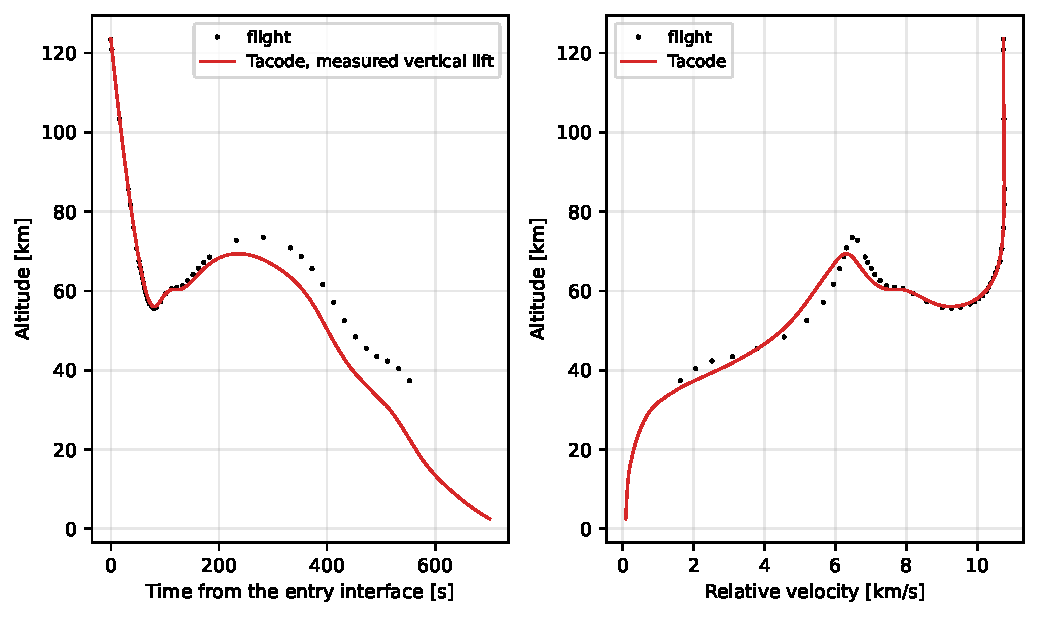
\includegraphics[width=0.95\linewidth]{apollo4_trajectory}
\end{center}
\caption{Apollo 4 with the measured vertical lift: altitude against time from the entry
interface (left) and the altitude-velocity plane (right).}
\label{apollo4_trajectory}
\end{figure}

\subsection{Apollo 10}

Apollo 10 is the case in which \textbf{nothing about the lift is assumed}. NASA TN D-6725
\cite{Graves1972} gives the state vector at the entry interface, the roll angle the guidance actually held
through the entry, and the altitude and velocity the vehicle actually flew. The roll angle
\emph{is} the direction of the lift, so it goes in as an input --- 89 nodes of a table
against time --- and the altitude and velocity are the comparison. Nothing is left to tune
except the entry mass, which is not in the reference.

Over the 311 digitised points spanning 12 to 414 s after the entry interface, the altitude
agrees to \textbf{3.2 km rms} (max $+5.5$ km) and the inertial velocity to 189 m/s rms
(Figure \ref{apollo10_trajectory}). That 3.2 km is the whole error budget of a
three-degree-of-freedom entry simulation: the atmosphere table, the constant coefficients,
the assumed mass, the digitisation of both the input and the reference, and the missing
degrees of freedom, all together.

A sensitivity sweep is what makes the number interpretable. Changing $C_L$ by $0.03$ ---
the accuracy the report itself claims for its preflight $L/D$ --- moves the altitude by
two to three times the baseline error, so \textbf{the lift coefficient is the limiting
input, not the solver}. The assumed mass is worth about 1 km per 10\,\%, and the time step
nothing at all. Turning the lift off costs 33 km rms, which is again the size of a missing
model rather than an accuracy.

\begin{figure}[h]
\begin{center}
	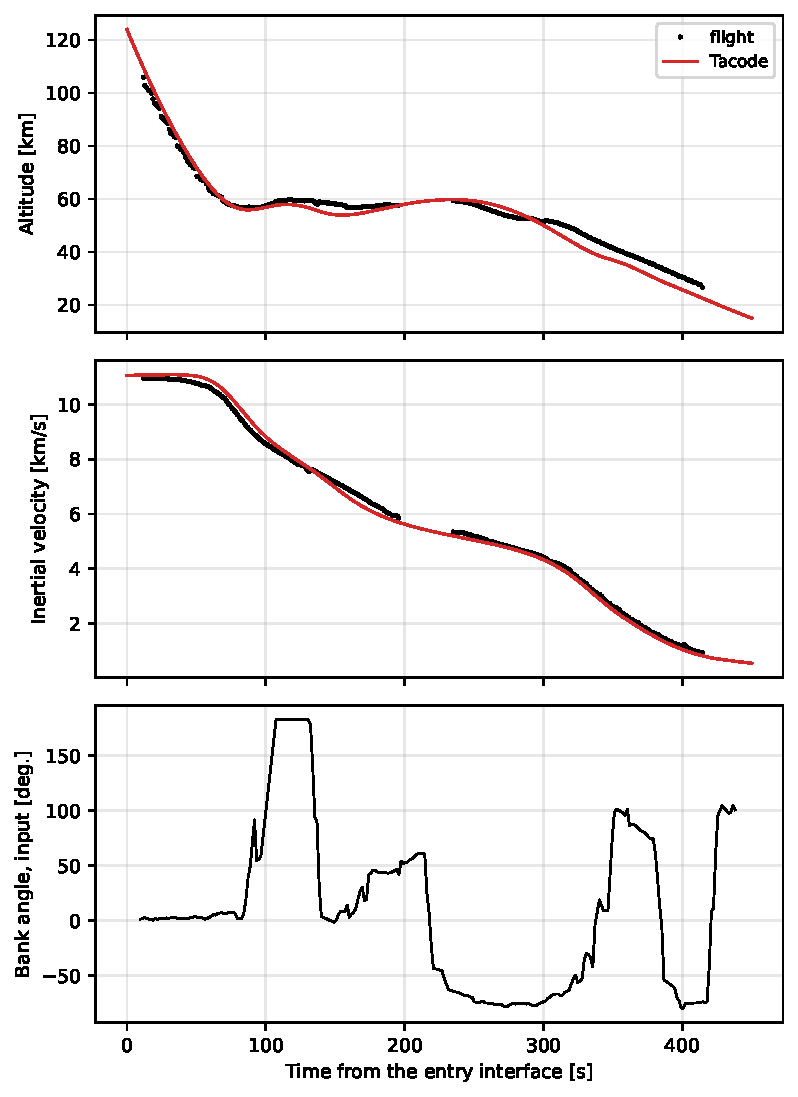
\includegraphics[width=0.55\linewidth]{apollo10_trajectory}
\end{center}
\caption{Apollo 10: altitude and inertial velocity against the flight, and the measured
bank angle that drives the case.}
\label{apollo10_trajectory}
\end{figure}

%----------------------------------------------------------------------
\subsection{Project Fire flight II} \label{fire2}

\subsubsection{Why this flight}

The two Apollo cases exercise the translational solver. Validating the \emph{attitude}
solver needs a flight with a published attitude measurement, and the constraints of the
code narrow the field sharply. Tacode has no control torque, so the vehicle must be
uncontrolled. Its aerodynamic table is indexed by the total angle of attack and the
Knudsen number but not by the Mach number, so the flight must stay in a regime where the
coefficients are insensitive to it. And the tabulated aerodynamics presume a body of
revolution, so a motion driven by asymmetry cannot be represented.

Those three rules eliminate the obvious candidates: the Apollo entries and every guided
entry vehicle by the first, ADEPT SR-1 and IRVE-3 by the second, Reentry F --- whose
published analysis is precisely about small mass and aerodynamic asymmetries --- by the
third. Stardust was uncontrolled and axisymmetric but its attitude was never measured.

Project Fire flight II survives all three. Launched on 1965-05-22 to study the radiative
heating of a blunt body returning from the Moon, its reentry package was spin-stabilised
at 171 rpm, completely uncontrolled, axisymmetric, and carried \textbf{three rate gyros
and three accelerometers} whose records are published \cite{Scallion1967}. It entered at
11 351 m/s on a $-14.7^\circ$ path.

\subsubsection{What the sources are}

Two reports are used, and it matters which layer of Table \ref{validation_cases} each
number belongs to.

\begin{itemize}
\item \textbf{NASA TN D-3569 table V} \cite{Lewis1966} is the trajectory, 625 records at
0.5 s intervals. Its title is ``Reentry trajectory parameters \emph{obtained from computer
simulation}'': it is NASA's own three-degree-of-freedom particle trajectory, started from
the Ascension Island radar at $t = 1608$ s and flown through an atmosphere measured by two
Nike-Apache sounding rockets. It is layer B. The report shows it merging with the radar
track on both sides of the telemetry blackout and reaching the measured impact point
within 500 m, so it is a good reference --- but agreeing with it checks the solver, not
the physics of the flight, and the extracted data file says so in its own header.
\item \textbf{NASA TN D-4183 figure 4} \cite{Scallion1967} gives the static coefficients
$C_X$, $C_R$ and $C_m$ against angle of attack, measured in the Ames hypersonic
free-flight facility at Mach 35. It is layer C, an input. It has a useful property: the
report itself used this figure to turn its flight rate-gyro records into angles of attack,
so the coefficients Tacode flies and the coefficients behind the ``measured'' angles of
attack are the same numbers.
\item \textbf{NASA TN D-4183 figures 17 and 19} are the attitude measurement, layer A, and
are treated in Section \ref{fire2_attitude}.
\end{itemize}

\subsubsection{Deciding in advance what can be checked}

This was written down before any number was computed, so that the write-up could not
become a selection of the intervals that happen to agree.

\emph{Can be checked}: the trajectory over the whole 312 s; the atmosphere table against
the sounding-rocket density; and the period of the pitch-yaw oscillation.

\emph{Cannot be checked}: the growth of the angle-of-attack envelope, because every step
of it was made by a discrete disturbance that Tacode has no way to represent; the decay of
the spin, for the same reason; and anything below about Mach 3, because neither the Tacode
table nor table V carries a Mach axis.

\subsubsection{Reading the data}

Table V is a numerical table, but it survives only as a 1966 scan whose embedded
optical character recognition drops digits, reads ``E'' as ``EUR'' and ``.'' as ``-'', and
shatters whole numbers into single characters. The extraction was written on one
principle: \textbf{nothing is filled in by interpolation}. A value that cannot be read is
written as \texttt{nan} and counted; 918 of the 7761 values are.

What \emph{can} be recovered is recovered from evidence. Three of the columns --- dynamic
pressure, pressure and density --- are printed twice, in SI and in US customary units,
which is a second independent reading of the same number; a value damaged in one unit is
recovered exactly from the other, and a pair that survives in both cross-checks itself. A
value whose magnitude is decades away from the median of its neighbours is a lost
exponent and goes. A minus sign that every neighbour contradicts, on a value whose
magnitude fits, is a lost character and is restored.

The layout is rebuilt from the coordinates of the text rather than from the character
stream, because the extraction tool walks a record column by column when its rows are far
apart. \textbf{Which of the three printed rows a value belongs to is decided by clustering
the vertical positions within each record, not by a fixed threshold}: some pages are
tilted enough that the right-hand columns of a row sit higher than its left-hand ones by
most of a row spacing, and a threshold there puts the density into the flight-path-angle
column. That fault cost a quarter of the density and temperature columns before it was
found.

The identities the table must satisfy are reported as a diagnostic and deliberately
\emph{not} used to reject values: $q_\infty = \rho V^2/2$ holds to a median of
$4 \times 10^{-7}$ and $M = V/a$ to $5 \times 10^{-6}$, while $p = \rho R T$ holds to
$2 \times 10^{-5}$ except above 95 km, where the composition changes and $R$ is no longer
287.05 --- a property of the table, not of the scan.

Figure 4 was digitised at 600 dpi. Its calibration is checked against the figure's own
grid lines, which land on their nominal values to 0.005 in $C_X$, 0.002 in $C_R$ and
0.0003 in $C_m$. \textbf{The origin of the angle-of-attack axis is not the left edge of the
frame}: the sixteen vertical grid lines are $5^\circ$ apart and the leftmost is $5^\circ$,
not $0$. Taking the frame for the origin shifts every coefficient by $5^\circ$, which puts
$C_D$ at 1.467 instead of 1.477 and --- far worse --- makes the small-angle slope of $C_m$
nearly twice as steep, because the first five degrees of that curve is where most of its
curvature lies. The error was not caught by eye but by physics: the oscillation frequency
of a six-degree-of-freedom run disagreed with the analytic result by a factor that pointed
straight at $C_{m\alpha}$. The corrected calibration puts $\alpha = 80^\circ$ within one
pixel of where the text layer of the document puts its ``80'' label. The digitised
coefficients are Figure \ref{fire2_aerodynamics}.

\begin{figure}[h]
\begin{center}
	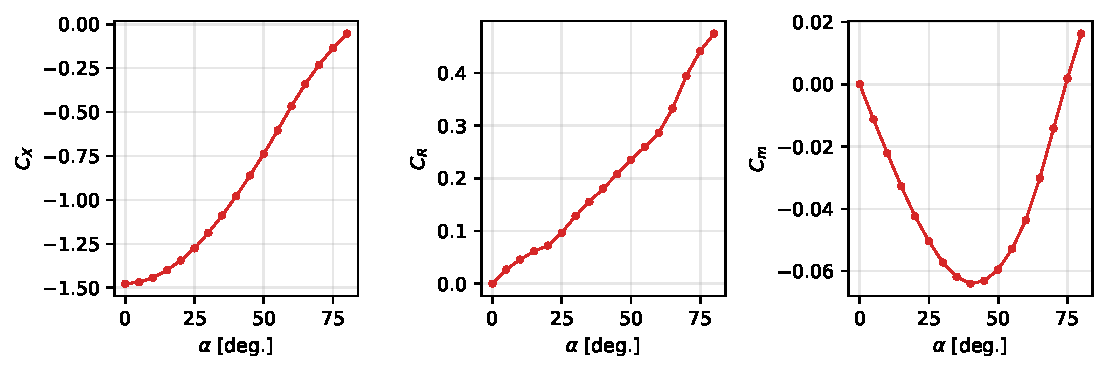
\includegraphics[width=0.98\linewidth]{fire2_aerodynamics}
\end{center}
\caption{Static aerodynamic coefficients of the Fire reentry package, digitised from
NASA TN D-4183 figure 4 (Ames hypersonic free-flight facility, Mach 35).
$C_D(0) = 1.4766$ and $C_{m\alpha} = -0.129$ per radian about the reference point of the
figure.}
\label{fire2_aerodynamics}
\end{figure}

\subsubsection{The vehicle, and why its ballistic coefficient is constant}

The reentry package shed three beryllium calorimeters and two phenolic-asbestos heat
shields during the entry, losing 24\,\% of its mass and 34\,\% of its pitch inertia
(Table \ref{fire2_mass}). A first reading of table V suggests that NASA ignored this,
because the ballistic coefficient can be read straight back out of the table --- it prints
both the dynamic pressure and the acceleration, so $C_D S/m = -a g / q_\infty$ --- and it
comes to $6.1490 \times 10^{-3}$ m$^2$/kg at every one of the 500 usable records, to four
figures.

They did not ignore it; the vehicle was built so that it did not matter.
\textbf{It sheds mass and frontal area in the same proportion.} Over the five
configurations the ballistic coefficient varies by $\pm 2.4$\,\% and $I_{yy}/d^3$, which
sets the attitude frequency, by $\pm 3.6$\,\%. A chain of runs that steps the mass, the
inertia and the diameter at the tabulated times moves the altitude agreement from 126 m to
124 m rms. That the step makes no difference is the result, and it is why a constant
ballistic coefficient was a fair choice in 1966.

\begin{table}[h]
\caption{Fire II reentry package: the five configurations of NASA TN D-4183 table I, with
the ballistic coefficient and the inertia parameter derived from them. The entry mass is
taken from TN D-3569 table III, 86.568 kg; TN D-4183 table I prints 86.586, but the
mass build-up of TN D-3569 table I ends at $94.73 - 8.16 = 86.57$ kg, which the former
rounds to and the latter does not.}
\label{fire2_mass}
\begin{center}
\begin{tabular}{l|r|r|r|r|r|r}
\hline \hline
Configuration & $t$, s & Mass, kg & $d$, m & $I_{yy}$, kg m$^2$ & $m/(\pi d^2/4)$ & $I_{yy}/d^3$ \\
\hline
Complete reentry package    & 1617.75 & 86.568 & 0.672 & 2.806 & 244.1 & 9.25 \\
Less first calorimeter      & 1640.48 & 83.189 & 0.651 & 2.644 & 249.9 & 9.58 \\
Less first phenolic layer   & 1642.12 & 76.022 & 0.630 & 2.305 & 243.9 & 9.22 \\
Less second calorimeter     & 1646.10 & 72.166 & 0.607 & 2.128 & 249.4 & 9.52 \\
Less second phenolic layer  & 1647.53 & 66.179 & 0.587 & 1.857 & 244.5 & 9.18 \\
\hline \hline
\end{tabular}
\end{center}
\end{table}

Because Tacode cannot change the vehicle in the middle of a run and its restart facility
is not implemented, the chain is driven from the case directory: each segment is run to
the next configuration change and the final state of its result file becomes the initial
condition of the next. Every quantity needed is already written in the convention the
control file wants. One trap is worth recording: the segments must be written out at every
step, because otherwise the last record falls short of the end of the segment by up to the
output interval, and half a second of a near-vertical descent is 700 m.

\subsubsection{Trajectory}

The entry state is taken from table V at $t = 1618.25$ s --- half a second after the
121 920 m entry interface, because the scan lost the latitude and longitude of the first
record --- and converted from the Earth-relative speed, flight-path angle and azimuth of
the table into the ECEF velocity in the geocentric local horizon.

Two runs are made. The first flies $C_D = 1.4766$, the value measured at Mach 35. The
second flies $C_D = 1.5009$, the value implied by table V's own ballistic coefficient,
which makes the \emph{input} identical so that what remains is the solver, the gravity
model and the atmosphere table. The difference between the two drag coefficients is
1.6\,\%. Results are in Table \ref{fire2_trajectory_results} and
Figure \ref{fire2_trajectory}.

\begin{table}[h]
\caption{Fire II: difference from table V, over the records where the scan preserved the
value. The hypersonic window ends at $t = 1700$ s, below which neither the Tacode table nor
table V carries a Mach axis.}
\label{fire2_trajectory_results}
\begin{center}
\begin{tabular}{l|l|c|c|c}
\hline \hline
Run & Window & Altitude & Relative velocity & Flight-path angle \\
\hline
$C_D = 1.4766$ (figure 4) & whole entry & max $+231$ m, rms 126 m & rms 12.2 m/s & rms $0.16^\circ$ \\
                          & hypersonic  & max $-179$ m, rms 117 m & rms 23.1 m/s & rms $0.11^\circ$ \\
$C_D = 1.5009$ (table V)  & whole entry & max $+333$ m, rms 182 m & rms 13.0 m/s & rms $0.16^\circ$ \\
                          & hypersonic  & max $-79$ m, rms \textbf{48 m} & rms 25.0 m/s & rms \textbf{$0.09^\circ$} \\
Mass stepped by segment   & whole entry & max $+217$ m, rms 124 m & rms 12.0 m/s & rms $0.17^\circ$ \\
\hline \hline
\end{tabular}
\end{center}
\end{table}

\textbf{With the input made identical, Tacode reproduces NASA's integration of the same
entry to 48 m rms in altitude and $0.09^\circ$ in flight-path angle} over the 82 s from
120 km to 20 km, through a peak deceleration of 73 $g$. That is $4 \times 10^{-4}$ of the
altitude, and it is the sharpest solver check in the set. The 117 m of the figure-4 run is
not solver error but the 1.6\,\% difference between two drag coefficients; which of them
is right is a question about a 1965 aerodynamic estimate. Below Mach 3 both runs drift by
a few hundred metres, which is the missing Mach dependence. The time step contributes
nothing: from $\Delta t = 0.005$ to $0.1$ s the altitude rms moves by 2 m.

\begin{figure}[h]
\begin{center}
	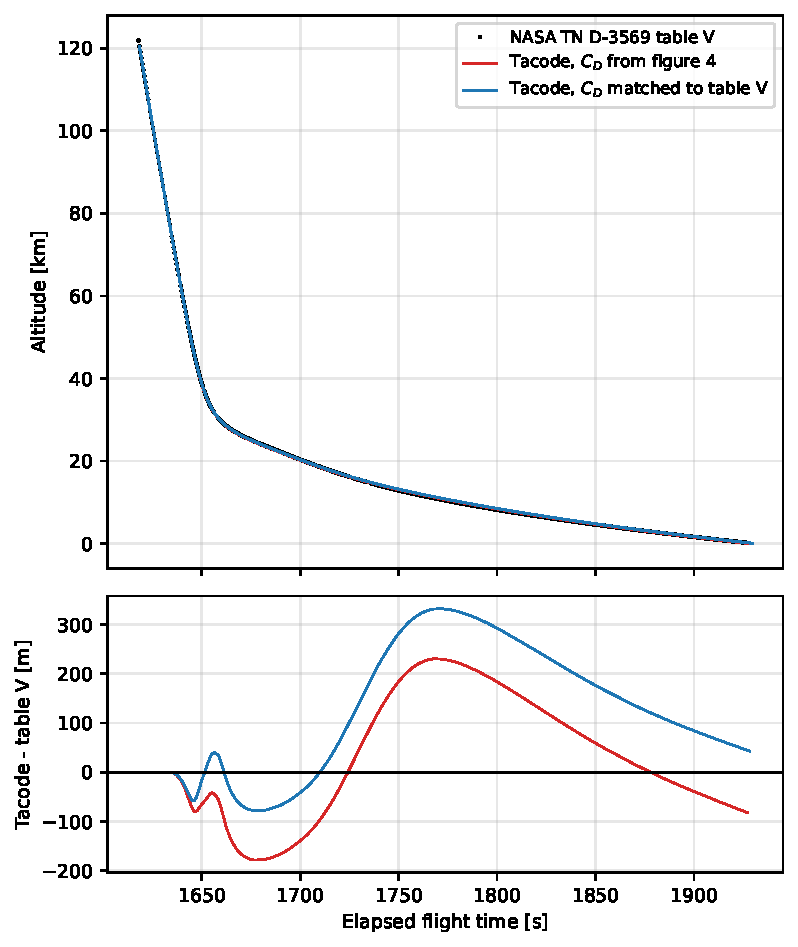
\includegraphics[width=0.58\linewidth]{fire2_trajectory}
\end{center}
\caption{Fire II trajectory against NASA TN D-3569 table V, and the residual.}
\label{fire2_trajectory}
\end{figure}

\subsubsection{Atmosphere}

Table V carries the ambient density, pressure and temperature of the atmosphere the
trajectory was flown through, which came from the two Nike-Apache soundings --- layer A.
Comparing it with the NRLMSISE-00 table Tacode flies does not involve the trajectory at
all (Table \ref{fire2_density_table}, Figure \ref{fire2_density}). The mean ratio is 0.994
with an rms scatter of 7.9\,\%. Below 60 km the two agree to 0.1\,\%, which is less a
triumph than a statement that both are close to a standard atmosphere there. The 25\,\% at
100 to 122 km is the thermosphere, where the solar indices matter --- $F_{10.7} = 75$ was
used for the May 1965 solar minimum because the indices of the day were not available
offline --- and where the dynamic pressure is below 2 N/m$^2$.

\begin{table}[h]
\caption{Fire II: the NRLMSISE-00 table against the density measured in flight.}
\label{fire2_density_table}
\begin{center}
\begin{tabular}{l|c|c|c|c|c|c|c}
\hline \hline
Altitude, km & all & 0--20 & 20--40 & 40--60 & 60--80 & 80--100 & 100--122 \\
\hline
Points & 535 & 392 & 91 & 15 & 11 & 12 & 14 \\
Mean ratio flight/table & \textbf{0.994} & 0.999 & 0.999 & 0.999 & 1.093 & 0.965 & 0.750 \\
\hline \hline
\end{tabular}
\end{center}
\end{table}

\begin{figure}[h]
\begin{center}
	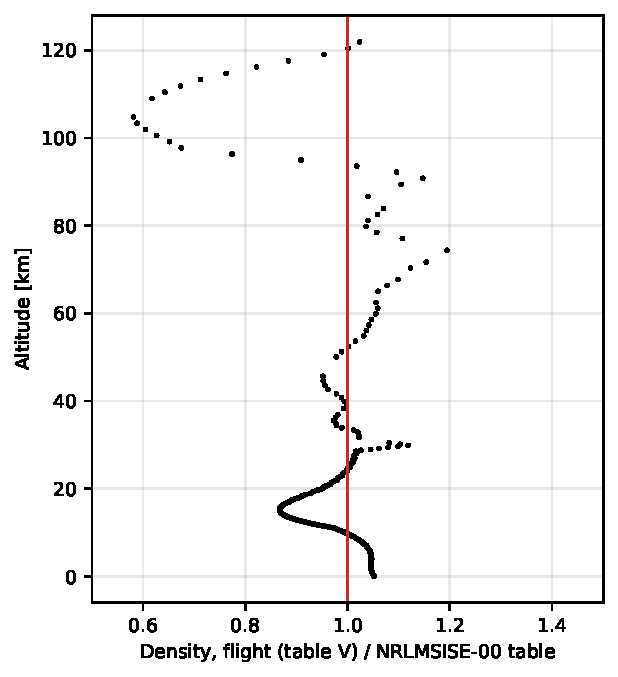
\includegraphics[width=0.42\linewidth]{fire2_density}
\end{center}
\caption{Fire II: ratio of the density measured by the Nike-Apache soundings to the
NRLMSISE-00 table the case flies.}
\label{fire2_density}
\end{figure}

\subsubsection{Attitude} \label{fire2_attitude}

Figure 17 of TN D-4183 plots two things: the dynamic pressure of the trajectory (dashed)
and \textbf{the dynamic pressure the report's own six-degree-of-freedom simulations needed
in order to match the frequency of the measured pitch and yaw rates} (solid, in short
segments). The report varied the dynamic pressure at the wind-tunnel value of
$C_{m\alpha}$ until the frequency matched, so those solid segments \emph{are} the measured
frequency, written as a dynamic pressure.

Turning that into a frequency requires the right relation, and for a spinning body it is
not Eq. (\ref{period}). The transverse motion of a spinning axisymmetric body splits into
two modes; taking the tricyclic solution \cite{Murphy1963} back into body axes, the slower
one appears at
%
\begin{align}
	\lambda = p - a + \sqrt{a^2 + k \, q_{\infty}} ,
	\qquad
	a = \frac{I_{xx} \, p}{2 I_{yy}} ,
	\qquad
	k = - \frac{ C_{m\alpha} S d }{ I_{yy} } .
	\label{tricyclic}
\end{align}
%
At zero dynamic pressure $\lambda = p$, which is simply the statement that an incidence
fixed in space is seen from the spinning body to rotate at the spin rate; it is a
different mode from the torque-free nutation, which appears at
$(I_{xx} - I_{yy}) p / I_{yy} = 4.5$ rad/s here. Confusing the two costs a factor in
$C_{m\alpha}$, and it did during this work.

The comparison script does not \emph{assume} Eq. (\ref{tricyclic}); it fits $k$ to the
Tacode run and reports how well the form holds, which is a verification in its own right:

\begin{itemize}
\item the relation fits 75 windows of the run to \textbf{0.05 rad/s rms} on frequencies of
27 to 46 rad/s, that is 0.15\,\%;
\item the fitted $k$ corresponds to $C_{m\alpha} = -0.1418$ per radian, against the
$-0.1423$ that the digitised table gives once its moment is transferred from the reference
point of the figure to the centre of gravity (the table alone gives $-0.1290$). The
aerodynamic table, the centre-of-gravity transfer and the rigid-body solver are therefore
mutually consistent to \textbf{0.4\,\%}.
\end{itemize}

Four of the six simulation windows of figure 17 separate cleanly from the dashed curve;
the other two lie on its steep flank. The comparison is Table \ref{fire2_frequency} and
Figure \ref{fire2_attitude_figure}.

\begin{table}[h]
\caption{Fire II: the oscillation frequency against the measured one. The primary quantity
is the ratio of the dynamic pressures; the frequencies are that ratio mapped through
Eq. (\ref{tricyclic}) with $k$ fitted to the Tacode run.}
\label{fire2_frequency}
\begin{center}
\begin{tabular}{c|r|r|c|r|r|c}
\hline \hline
Window, s & $q_\infty$ Tacode, N/m$^2$ & $q_\infty$ required, N/m$^2$ & ratio &
$\omega$ computed, rad/s & $\omega$ measured, rad/s & ratio \\
\hline
1644.9 &  66\,652 &  67\,569 & 1.014 & 37.17 & 37.35 & 1.005 \\
1649.3 & 117\,344 & 133\,438 & 1.137 & 45.93 & 48.33 & \textbf{1.052} \\
1652.6 & 108\,241 & 112\,185 & 1.036 & 44.51 & 45.13 & 1.014 \\
1662.4 &  26\,337 &  26\,156 & 0.993 & 27.74 & 27.69 & 0.998 \\
\hline \hline
\end{tabular}
\end{center}
\end{table}

\textbf{The oscillation Tacode predicts is within 5\,\% of the one the vehicle flew} ---
1.7\,\% on average over the four windows, with the largest error at the peak of the
dynamic pressure. The run through the segmented configurations gives the same answer to
0.2\,\%.

That 5\,\% is close to the resolution of the test. The report attributes the gap between
the two curves of its own figure 17 to ``uncertainties in the atmospheric measurements or
the wind-tunnel data, or both'', and the digitisation of that figure is itself worth about
600 N/m$^2$ rms --- which is how well its dashed curve reproduces the dynamic pressure of
table V, and therefore how well the calibration is known.

\begin{figure}[h]
\begin{center}
	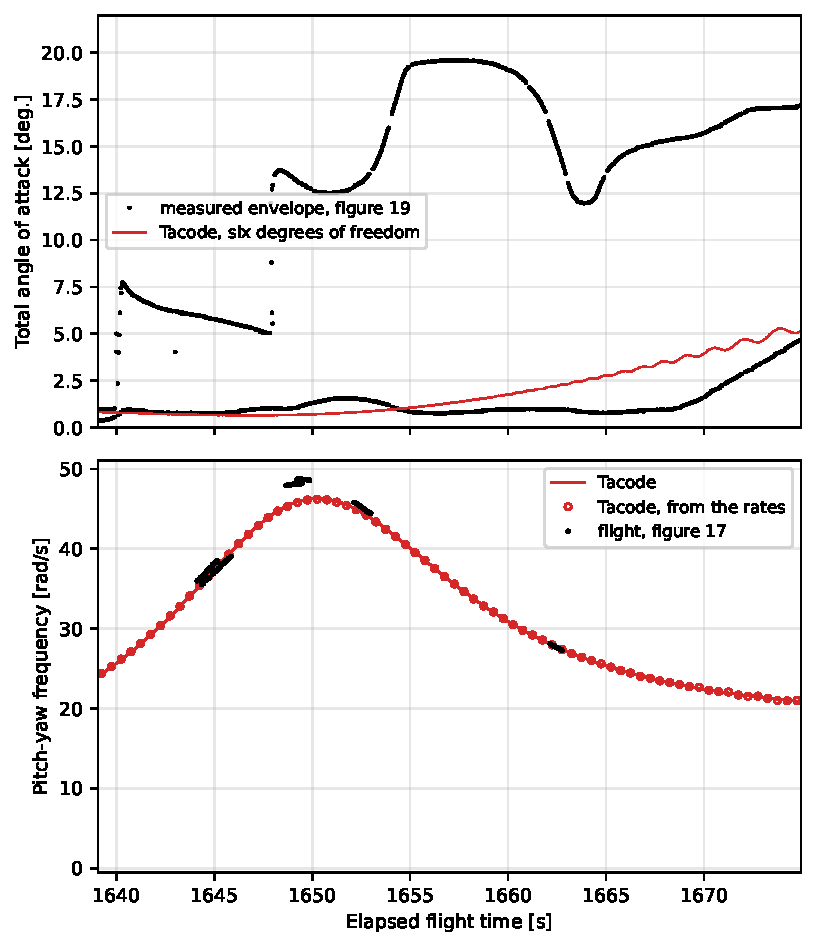
\includegraphics[width=0.58\linewidth]{fire2_attitude}
\end{center}
\caption{Fire II attitude. Top: the total angle of attack against the measured envelope of
figure 19 --- these are \emph{not} comparable, and the figure is drawn to show the size of
what is missing. Bottom: the pitch-yaw frequency.}
\label{fire2_attitude_figure}
\end{figure}

\subsubsection{What is deliberately not compared}

Over the interval figure 19 covers, Tacode's total angle of attack stays between
$0.64^\circ$ and $5.29^\circ$ while the measured envelope climbs from $0.36^\circ$ to
$19.59^\circ$. \textbf{No error is quoted for that, because the two are not comparable.}
The measured envelope is a staircase and every step is a disturbance: the first beryllium
calorimeter melting asymmetrically at $t = 1640.38$ s (an angular impulse of
6.440 N m s), the second phenolic heat shield coming off at 1648.18 s (9.49 N m s), and a
series of events from 1652.7 s that the report itself could not identify. Tacode has no
way to represent any of them.

The angular impulses \emph{could} have been put in --- the report measures their magnitude
--- but not their direction. A run that reproduced the envelope would have had that
direction chosen to make it do so, which is fitting and not validation. For the same
reason the chained runs step only the mass, the inertia and the diameter, and the spin is
held constant although the flight lost half of it between $t = 1658$ and 1662 s through a
disturbance the report could not explain either.

Three figures of the reports were examined and deliberately not digitised, and the scripts
record why: figure 8 of TN D-4183, because the roll-rate samples scatter too far and the
report prints the numbers in its text; figure 9, because its symbols overlap so far that
only 30 of some 200 can be separated and those 30 sit in the sparser stretches, which
would make a biased sample; and figure 17 of TN D-3569, the radar comparison, because
three quantities and four tracking systems overlap in it at a reading accuracy of about
1.5 km in altitude --- ten times coarser than the agreement being measured.

%----------------------------------------------------------------------
\section{Example Results}

Figures \ref{example_orbit} to \ref{example_reentry_6dof} show the three tutorial cases
distributed with the code: a 5000 s low orbit, a ballistic re-entry, and the same re-entry
solved in six degrees of freedom. They are also the regression cases, so their outputs are
committed with the code and reproduced to a relative $10^{-9}$ by the test suite.

\begin{figure}[h]
\begin{center}
	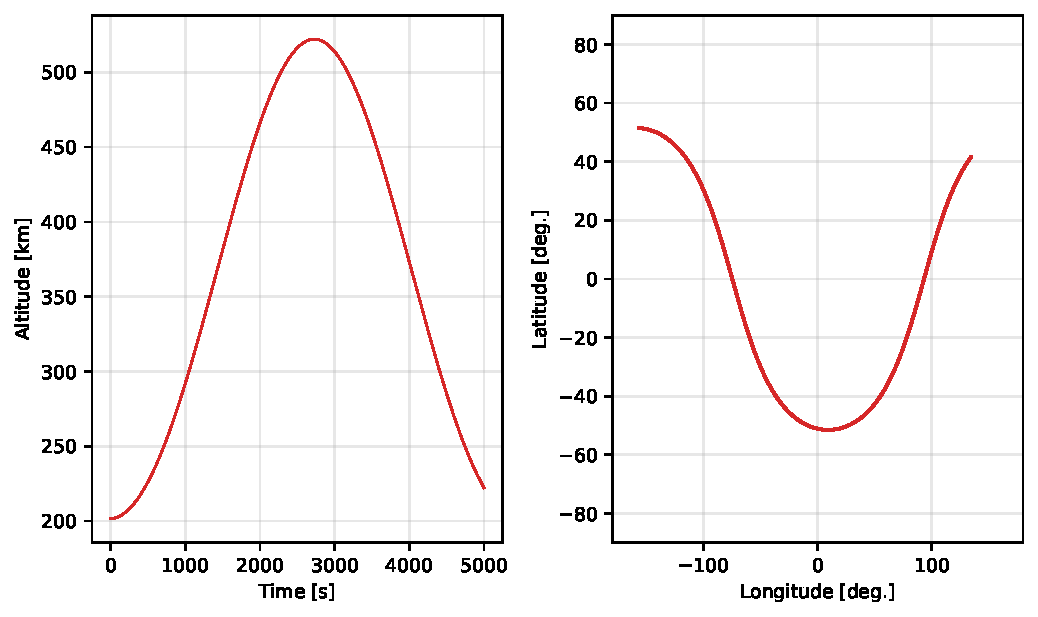
\includegraphics[width=0.85\linewidth]{example_orbit}
\end{center}
\caption{Tutorial case \texttt{work}: a low Earth orbit over 5000 s. Altitude against time
(left) and the ground track (right).}
\label{example_orbit}
\end{figure}

\begin{figure}[h]
\begin{center}
	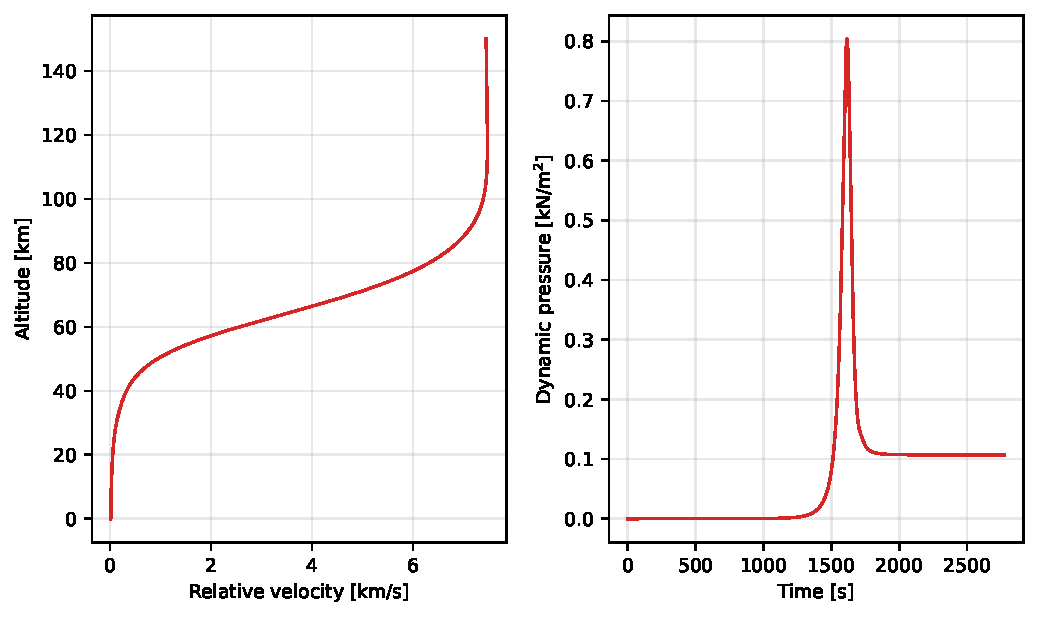
\includegraphics[width=0.85\linewidth]{example_reentry}
\end{center}
\caption{Tutorial case \texttt{work\_reentry}: a ballistic re-entry. The altitude-velocity
plane (left) and the dynamic pressure (right).}
\label{example_reentry}
\end{figure}

\begin{figure}[h]
\begin{center}
	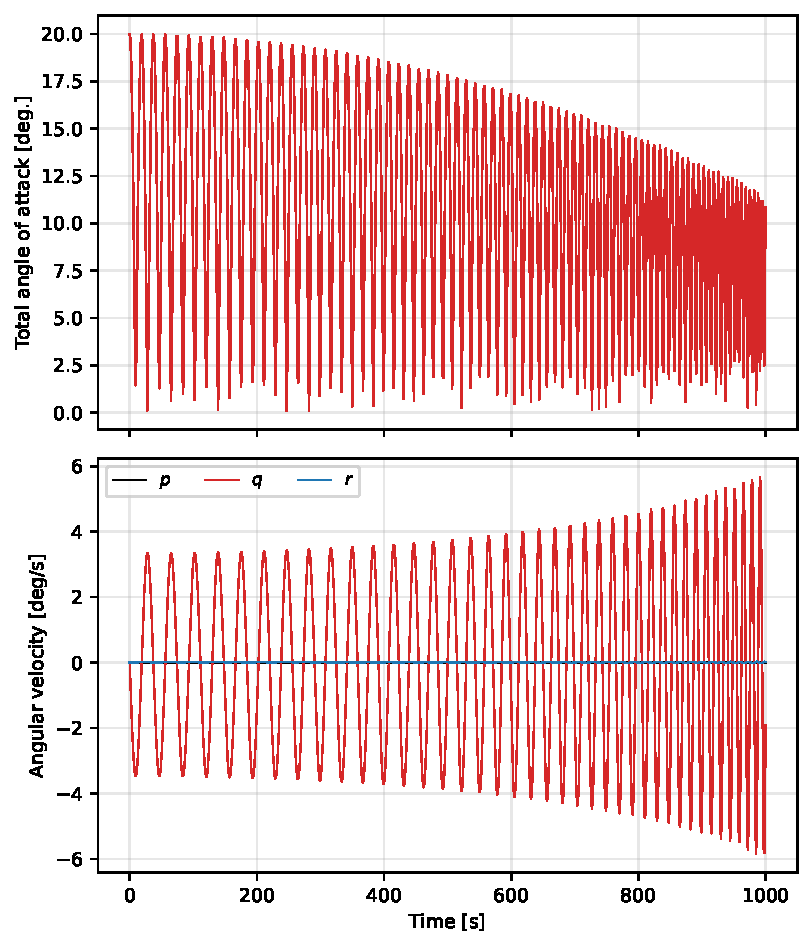
\includegraphics[width=0.55\linewidth]{example_reentry_6dof}
\end{center}
\caption{Tutorial case \texttt{work\_reentry\_6dof}: the same entry with the attitude
solved. The total angle of attack (top) and the body-axis angular velocity relative to
ECEF (bottom). The oscillation frequency rises with the dynamic pressure, as
Eq. (\ref{period}) requires.}
\label{example_reentry_6dof}
\end{figure}

%----------------------------------------------------------------------
\section{Summary}

Version 2 of Tacode extends the point-mass formulation of version 1 with the rotational
degrees of freedom of a rigid body, a lift force whose direction is set by a prescribed
bank angle, a wind field, an absolute time, and detection of a diverged run. Every one of
those is off by default, and with it off the output is unchanged byte for byte, which the
regression tests enforce; that constraint is a deliberate design rule, not an accident.

Correctness is established at two levels. Verification --- 488 automated tests built on
closed-form solutions, physical identities, mutation testing and byte-for-byte regression
--- establishes that the equations are solved as written, and the observed order of
convergence of the integrator is 4.3 and 3.9 for the translational and the rotational
state on a case with a 73 $g$ deceleration.

Validation against three flights establishes what the equations are worth. Apollo 4 and
Apollo 10 exercise the translational solver against lifting entries with the lift
direction taken from the flight; the better conditioned of the two, Apollo 10, agrees to
3.2 km rms in altitude over a 414 s entry, with the lift coefficient rather than the
solver as the limiting input. Project Fire flight II, an uncontrolled spin-stabilised
entry, exercises the attitude solver: with the same drag coefficient the trajectory
reproduces NASA's own integration to 48 m rms, the atmosphere table matches the
sounding-rocket density to 0.6\,\% in the mean, and \textbf{the predicted pitch-yaw
oscillation is within 5\,\% of the one the vehicle flew}, which is close to the resolution
of the available measurement.

Equally a part of the result is what was decided \emph{not} to compare, and why: the
growth of the Fire II angle-of-attack envelope, which was driven by disturbances whose
direction is not published; the Apollo 4 drag-only trajectory, whose 27 km is the size of
a missing model rather than an accuracy; and three figures whose reading accuracy is
coarser than the quantity being measured. A validation report is only as good as its
account of its own limits.

%----------------------------------------------------------------------
\begin{thebibliography}{9}

\bibitem{Wagner1966}
C.~A. Wagner,
``The Gravity Potential and Force Field of the Earth Through Fourth Order'',
{\em NASA TN D-3317}, 1971.

\bibitem{Liu2019}
F.~Liu, S.~Lu and Y.~Sun,
{\em Guidance and Control Technology of Spacecraft on Elliptical Orbit},
Springer, 2019.

\bibitem{Lewis1966}
J.~H. Lewis, Jr. and W.~I. Scallion,
``Flight Parameters and Vehicle Performance for Project Fire Flight II, Launched
May 22, 1965'',
{\em NASA TN D-3569}, 1966.

\bibitem{Scallion1967}
W.~I. Scallion and J.~H. Lewis, Jr.,
``Body Motions and Angles of Attack During Project Fire Flight II Reentry'',
{\em NASA TN D-4183}, 1967.

\bibitem{Murphy1963}
C.~H. Murphy,
``Free Flight Motion of Symmetric Missiles'',
{\em Ballistic Research Laboratories Report No. 1216}, 1963.

\bibitem{Hillje1969}
E.~R. Hillje,
``Entry Aerodynamics at Lunar Return Conditions Obtained from the Flight of Apollo 4
(AS-501)'',
{\em NASA TN D-5399}, 1969.

\bibitem{Ried1972}
R.~C. Ried, Jr., W.~C. Rochelle and J.~D. Milhoan,
``Radiative Heating to the Apollo Command Module: Engineering Prediction and Flight
Measurement'',
{\em NASA TM X-58091}, 1972.

\bibitem{Graves1972}
C.~A. Graves, Jr. and J.~C. Harpold,
``Apollo Experience Report --- Mission Planning for Apollo Entry'',
{\em NASA TN D-6725}, 1972.

\end{thebibliography}

\end{document}
